%%
%%    ToolBus -- The ToolBus Application Architecture
%%    Copyright (C) 1998-2000  Stichting Mathematisch Centrum, Amsterdam, 
%%                             The  Netherlands.
%%
%%    This program is free software; you can redistribute it and/or modify
%%    it under the terms of the GNU General Public License as published by
%%    the Free Software Foundation; either version 2 of the License, or
%%    (at your option) any later version.
%%
%%    This program is distributed in the hope that it will be useful,
%%    but WITHOUT ANY WARRANTY; without even the implied warranty of
%%    MERCHANTABILITY or FITNESS FOR A PARTICULAR PURPOSE.  See the
%%    GNU General Public License for more details.
%%
%%    You should have received a copy of the GNU General Public License
%%    along with this program; if not, write to the Free Software
%%    Foundation, Inc., 59 Temple Place, Suite 330, Boston, MA  02111-1307 USA
%%
\documentclass[a4paper,twoside]{article} % -*-latex-*-
\setlength{\oddsidemargin}{0.235cm}
\setlength{\evensidemargin}{0.235cm}
\setlength{\textwidth}{16cm}
\topmargin 0.5cm  % was: 0.2cm
\pagestyle{myheadings}


\usepackage{epsfig}
\usepackage{a4wide}

\begin{document}

\newcommand{\TB}{{\sc ToolBus}}
\newcommand{\T}{{\bf T}}
\newcommand{\spec}[1]{{\rm #1}}
\newcommand{\script}[1]{{\tt #1}}
\newcommand{\ASFSDF}{{\sc Asf+Sdf}}
\newcommand{\ASF}{{\sc Asf}}
\newcommand{\SDF}{{\sc Sdf}}
\newcommand{\GEL}{{\sc Gel}}
\newcommand{\iter}{\,^*\,}
\newcommand{\emp}[1]{{\em #1}}
\newcommand{\txttt}[1]{{\tt #1}}

\title{A \TB\ introduction \\
Version 0.1}
\author{P.A. Olivier$^{1}$}
\date{\today}
\maketitle
\begin{center}
       {\footnotesize $^1$ Programming Research Group, University of Amsterdam\\
        P.O. Box 41882, 1009 DB Amsterdam, The Netherlands}
\end{center}

\begin{abstract}

The \TB\ is a new software architecture intended for building
cooperating, distributed applications.  This document aims
at providing an easy to use introduction to using and programming
the ToolBus.
\end{abstract}

\tableofcontents

\newpage

\section{First steps}

To use the \TB, you first have to find it. There are two important
locations to locate: the location of the \TB\ executable, and the
location of the \TB\ distribution, wich contains the demos.

By the time you are reading this document, you have probably already
found the ToolBus distribution, because this document is part of it.

The first thing to do, is locating the \TB\ executable. It is usually
called {\tt toolbus}, so you can try using the command {\tt which toolbus}
to see if the {\tt toolbus} executable is already in your
search path:

\begin{verbatim}
olivierp@gene 180> which toolbus
/home/gipe/petr/bin/toolbus
olivierp@gene 181>
\end{verbatim}

If this is not the case, your best bet might be to try the {\tt bin}
directory of the \TB\ distribution from which you got this document.
Or you might try to use the {\tt locate} command
to find its location:
\begin{verbatim}
olivierp@gene 185> locate toolbus | grep bin
/nfs/gene/gen3/gipe/petr/bin/toolbus
\end{verbatim}

When you have found the {\tt toolbus} executable, and it is not yet
in your search path, you might want to add it. If you do not know how
to do this, consult somebody with a basic understanding of the
unix shell, like your system administrator.

Now start the \TB\ with the {\tt -v} option, to test your setup,
and to see which version of the \TB\ you are using:

\begin{verbatim}
olivierp@gene 186> toolbus -version
version: ToolBus-0.9.19
olivierp@gene 187>
\end{verbatim}

You are all set, and ready to go!

\section{The {\tt calc} demo}

We will show some of the \TB\ features using the simple {\tt calc} demo.
First, {\tt cd} to the directory {\tt demos/calc} in the \TB\ distribution.
Now start the calculator demo by issuing the following command:

\begin{verbatim}
toolbus calc.tb
\end{verbatim}

\begin{figure}[htb]
\centerline{
\epsfig{file=calc-ui.eps}}
\caption{The calculator user interface}
\label{calc-ui}
\end{figure}

If anything goes wrong, please refer to the appendix 
\ref{trouble} (Trouble shooting).
The calculator user interface comes up as shown in Figure \ref{calc-ui}.
Pressing the {\tt Calc} button pops up a new window to ask you to enter
an expression like {\tt plus(3,times(2,5))}.
When you are done entering this expression, just press 
\verb@<Return>@, and the result will pop up in another window.

Pressing the {\tt showLog} button will popup a window showing the
expressions calculated so far, including expressions calculated
by a hidden {\tt batch} tool.


The {\tt showTime} button can be used to display the current time.
You can use the {\tt Quit} button to end the demo.

\subsection{The calculator \TB\ configuration}

Figure \ref{calc-impl} shows the calculator demo \TB\ configuration.
The calculator demo consists of four tools:

\begin{figure}[htb]
\centerline{\epsfig{file=calc.ps}}
\caption{The calculator \TB\ configuration}
\label{calc-impl}
\end{figure}

\begin{itemize}
\item The {\tt clock} tool delivers the current time on request.
\item The {\tt ui} tool implements the user interface of the calulator demo.
\item The {\tt calc} tool calculates the values of expressions.
\item The {\tt batch} tool generates expressions at random time intervals.
\end{itemize}

The communication between these four tools is controlled by five processes:
\begin{itemize}
\item The {\tt CLOCK} process catches requests for the current time,
      relays them to the {\tt clock} tool, and sends the answer back.
\item The {\tt UI} process waits for user actions, and translates
      them into requests to the {\tt CLOCK}, {\tt CALC}, or {\tt LOG}
      process.
\item The {\tt CALC} process waits for expression calculation requests,
      calculates the value of the expression, and sends the result back.
      This process also broadcasts the expression/result pairs.
\item The {\tt LOG} process waits on broadcasted expression/result pairs,
      and logs them in a list.
      On request, the {\tt LOG} process can send this complete log of
      evaluated expressions.
\item The {\tt BATCH} process waits for evaluation requests from the
      batch tool, and relays them to the {\tt CALC} process.
\end{itemize}

\subsection{The calculator \TB\ script}
\small
\begin{verbatim}
process CALC is
  let Tid : calc, E : str, V : term
  in
     execute(calc, Tid?) .
     ( rec-msg(compute, E?) . snd-eval(Tid, expr(E)) .
       rec-value(Tid, V?) .
       snd-msg(compute, E, V) . snd-note(compute(E, V))
     ) * delta
  endlet

\end{verbatim}
\noindent
\normalsize
 We take a closer look at the definition of the \script{CALC} process.
 First, three typed variables are introduced: \script{Tid} (of type \script{calc},
 a tool identifier representing the \script{calc}-tool, see below),
 \script{E} (a string variable representing the expression whose value is to be computed),
 and \script{V} (an integer variable representing the computed value of expressions).
 The first atom,
 \begin{quote}
 \script{execute(calc, Tid?)}
 \end{quote}
 executes the \script{calc}-tool using the
 command (and optionally also the desired host computer)
 as defined in \script{calc}'s tool definition.  The
 result variable \script{Tid} gets as value a descriptor of
 this particular execution of the \script{calc}-tool. All
 subsequent atoms (e.g., \script{snd-eval}, \script{rec-event})
 that communicate with this tool instance will use this descriptor as
 first argument. Next, we encounter a construct of the form
 \begin{quote}
 ( rec-msg(compute, E?)
   ...
 ) * delta
 \end{quote}
 describing an infinite repetition of all steps inside the parentheses.
 Note that inaction (\script{delta}) will be avoided as long as there
 are other steps possible.
 Next, we see the atom
 \begin{quote}
 \script{rec-msg(compute, E?)}
 \end{quote}
 for receiving a computation request from another process. Here, \script{compute}
 is a constant, and the variable \script{E} will get as value a string
 representing the expression to be computed. Next, an evaluation request
 goes to the \script{calc}-tool as a result of
 \begin{quote}
 \script{snd-eval(Tid, expr(E))}
 \end{quote}
 The resulting value is received by
 \begin{quote}
 \script{rec-value(Tid, V?)}
 \end{quote}
 Observe the combination of an ordinary variable \script{Tid} and
 a result variable \script{V}.  Clearly, this atom should {\em only}
 match with a value event coming from the \script{calc}-tool that was
 executed at the beginning of the \script{CALC} process.  It is also
 clear that \script{V} should get a value as a result of the match.
 A reply to the original request \script{rec-msg(compute, E?)} is then given by
 \begin{quote}
 \script{snd-msg(compute, E, V)}
 \end{quote}
 and this is followed by the notification
 \begin{quote}
 \script{ snd-note(compute(E, V))}
 \end{quote}
 that will be used by the \script{LOG} process.

 \noindent The definition for the \script{calc} tool is:

\small
\begin{verbatim}
tool calc is {command = "./calc"}

\end{verbatim}
\noindent
\normalsize
 The string value given for \script{command} is the operating system level
 command needed to execute the tool. It may contain additional arguments
 as can be seen in the definition of the \script{ui}-tool below.

 The user-interface is defined by the
 process \script{UI}. First, it executes the \script{ui}-tool and then
 it handles three kinds of buttons.
 Note that the buttons ``calc'' and ``log'' exclude each other:
 either the ``calc'' button or the ``log'' button may be pushed but not both at the same time.
 The ``time'' button is independent of the other two buttons: it remains enabled
 while any of the other two buttons has been pushed.

\small
\begin{verbatim}
process UI is
  let Tid : ui
  in
     execute(ui, Tid?) .
     ( ( CALC-BUTTON(Tid) + LOG-BUTTON(Tid) ) * delta
     ||
       TIME-BUTTON(Tid) * delta
     ||
       QUIT-BUTTON(Tid)
     )
  endlet

tool ui is {command = "wish-adapter -script ui-calc.tcl"}

\end{verbatim}
\noindent
\normalsize
 The treatment of each button is defined in a separate, auxiliary,
 process definition. They have a common structure:
 \begin{itemize}
 \item Receive an event from the user-interface.
 \item Handle the event (either by doing a local
 computation or by communicating with other \TB\ processes that may
 communicate with other tools).
 \item Send an acknowledgement to the user-interface that the handling
 of the event is complete.
 \end{itemize}

\small
\begin{verbatim}
process CALC-BUTTON(Tid : ui) is
  let  N : int, E : str, V : term
  in
     rec-event(Tid, N?, button(calc)) .
     snd-eval(Tid, get-expr-dialog).
     ( rec-value(Tid, cancel)
     + rec-value(Tid, expr(E?)) .
       snd-msg(compute, E) . rec-msg(compute, E, V?) .
       snd-do(Tid, display-value(V))
     ) . snd-ack-event(Tid, N)
  endlet

process LOG-BUTTON(Tid : ui) is
  let N : int, L : term
  in
      rec-event(Tid, N?, button(showLog)) .
      snd-msg(showLog) .  rec-msg(showLog, L?) .
      snd-do(Tid, display-log(L)) .
      snd-ack-event(Tid, N)
  endlet

process TIME-BUTTON(Tid : ui) is
  let N : int, T : str
  in
      rec-event(Tid, N?, button(showTime)) .
      snd-msg(showTime) . rec-msg(showTime, T?) .
      snd-do(Tid, display-time(T)) .
      snd-ack-event(Tid, N)
  endlet

process QUIT-BUTTON(Tid : ui) is
  rec-event(Tid, button(quit)) .
  shutdown("End of calc demo")


\end{verbatim}
\noindent
\normalsize
 The \script{BATCH} process executes the \script{batch} tool,
 reads expressions from file, computes their value by exchanging messages
 with process \script{CALC} and writes an (expression, value) pair
 back to a file.

\small
\begin{verbatim}
process BATCH is
  let Tid : batch, E : str, V : int
  in
     execute(batch, Tid?) .
     ( snd-eval(Tid, fromFile). rec-value(Tid, expr(E?)) .
       snd-msg(compute, E). rec-msg(compute, E, V?).
       snd-do(Tid, toFile(E, V))
     ) * delta
  endlet

tool batch is {command = "./batch"}

\end{verbatim}
\noindent
\normalsize
 The \script{LOG} process subscribes to notes of the form \script{compute(<str>,<int>)},
 i.e., a function \script{compute} with a string and an integer as arguments.

\small
\begin{verbatim}
process LOG is
  let Tid : log, E : str, V : term, L : term
  in
     subscribe(compute(<str>,<term>)) .
     execute(log, Tid?) .
     ( rec-note(compute(E?, V?)) . snd-do(Tid, writeLog(E, V))
     + rec-msg(showLog) . snd-eval(Tid, readLog) .
       rec-value(Tid, L?) . snd-msg(showLog, L)
     ) * delta
  endlet

tool log is {command = "./log"}

\end{verbatim}
\noindent
\normalsize
 There are alternatives for the way in which the process definitions
 in this example can be defined. The \script{LOG} process can, for instance,
 be defined without resorting to a tool in the following manner:

\small
\begin{verbatim}
process LOG1 is
  let TheLog : list, E : str, V : term
  in
     subscribe(compute(<str>,<term>)) .
     TheLog := [] .
     ( rec-note(compute(E?, V?)) . TheLog := join(TheLog, [[E, V]])
     + rec-msg(showLog) .  snd-msg(showLog, TheLog)
     ) * delta
  endlet

\end{verbatim}
\noindent
\normalsize
 Instead of storing the log in a tool we can use a variable (\script{TheLog})
 for this purpose in which we maintain a list of pairs. We use
 the function ``\script{join}'' (list concatenation) to append a new pair
 to the list. Note that \script{join} operates on lists, hence we concatenate
 a singleton list consisting of the pair as single element.
 The process \script{CLOCK} executes the \script{clock} tool and answers
 requests for the current time.

\small
\begin{verbatim}
process CLOCK is
  let Tid : clock, T : str
  in
     execute(clock, Tid?) .
     ( rec-msg(showTime) .
       snd-eval(Tid, readTime) .
       rec-value(Tid, T?) .
       snd-msg(showTime, T)
     ) * delta
  endlet

tool clock is {command = "./clock"}

\end{verbatim}
\noindent
\normalsize
 Finally, we define one of the possible \TB\ configurations that can be defined
 using the above definitions:

\small
\begin{verbatim}
toolbus(UI, CALC, LOG1, CLOCK, BATCH)
\end{verbatim}
\normalsize


\section{The auction demo}

Now we come to the {\tt auction} demo. {\tt cd} to the directory
{\tt demos/auction} in the \TB\ distribution. Start the calculator
demo by issuing the following command:

\begin{verbatim}
toolbus auction.tb
\end{verbatim}

\begin{figure}[htb]
\centerline{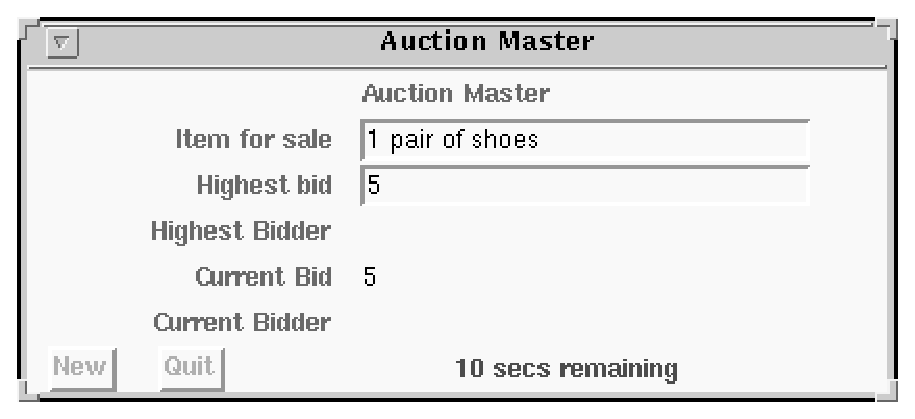
\epsfig{file=auction-master.eps}}
\caption{The auction master}
\label{auction-master}
\end{figure}

This will start the auction master, shown in Figure \ref{auction-master}. 
You can start different bidders (Figure \ref{auction-bidder})
like this:

\begin{verbatim}
bidder Pieter
\end{verbatim}

If you want a bidder to connect to an auction on a different machine,
and possibly a different port, you type something like:

\begin{verbatim}
bidder Pieter adam 8999
\end{verbatim}

\begin{figure}[htb]
\centerline{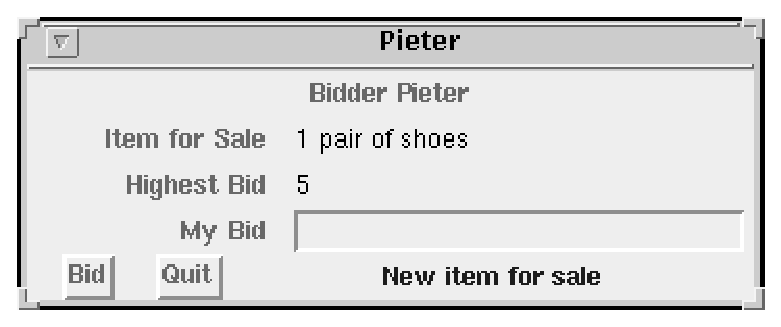
\epsfig{file=auction-bidder.eps}}
\caption{A bidder}
\label{auction-bidder}
\end{figure}

The auction begins when the auction master presses the {\tt New}
button after entering an item for sale and the starting `highest
bid'. The bidders can now freely bid, until nobody has makes a new
bid for ten seconds. At this time, everybody is notified that the bidding is
about to end. If nobody reopens the bidding in another ten seconds,
the item is sold to the highest bidder.

\subsection{The auction \TB\ configuration}


Figure \ref{auction-impl} shows the auction demo \TB\ configuration.
The demo consists of two different tools:

\begin{itemize}
\item The {\tt master} tool represents the auction master. Only one
 of these can be present at any one time.
\item The {\tt bidder} tool implements the bidder user interface.
      Any number of bidders can be present. Bidders can enter and leave
      the auction when they want.
\end{itemize}

\begin{figure}[htb]
\centerline{\epsfig{file=auction.ps}}
\caption{The auction demo \TB\ configuration}
\label{auction-impl}
\end{figure}


The communication between these four tools is controlled by two processes:
\begin{itemize}
\item The {\tt Auction} process regulates the auction demo. 
      It connects new bidders,
      and controls the auction of items.
\item The{\tt Bidder} processes control individual bidders.
      For every new bidder, the {\tt Auction} process creates a new
      {\tt Bidder} process to control this new bidder.
\end{itemize}


\subsection{The auction \TB\ script}
\input{auction.tb.tex}

\appendix
\section{Trouble shooting}
\label{trouble}

\noindent
{\bf Q: I am trying to start the \TB\, but get the following error message:}
\begin{verbatim}
ToolBus: cannot connect, giving up (Address already in use)
\end{verbatim}
A: This message can be caused by two things:
\begin{enumerate}
\item Some (unix) processes of an earlier \TB\ session is still running.
Use the {\tt ps} command to locate the offending processes, and kill them
using the {\tt 'kill $pid$'} command.
\item Somebody else is running a \TB\ session on the same machine, and on
the same port. Choose another port using the {\tt -TB\_PORT} option:
\begin{verbatim}
mel:~/ToolBus/demos/calc> toolbus -TB_PORT calc.tb
\end{verbatim}
\end{enumerate}

\noindent{\bf Q: When I start the \emph{...} demo,
the system crashes immediately with approximately the following output:}
\begin{verbatim}
mel:~/ToolBus/demos/calc> tb calc.tb
     ToolBus -- UNEXPECTED INPUT snd-disconnect(ui(0)) FROM TOOL tool-inst(ui,0
,6,6,"mel",2,[]) IGNORED
cnt = -1
ToolBus: multi_read, cannot read (Interrupted system call)
ToolBus: tool-inst(ui,0,6,6,"mel",2,[]): read failed (Interrupted system call)
cnt = -1
ToolBus: multi_read, cannot read (Interrupted system call)
ToolBus: tool-inst(ui,0,6,6,"mel",2,[]): read failed (Interrupted system call)
cnt = -1
ToolBus: multi_read, cannot read (Interrupted system call)
ToolBus: tool-inst(ui,0,6,6,"mel",2,[]): read failed (Interrupted system call)
ToolBus: read_term: cannot find ready input channel
cnt = -1
clock: multi_read, cannot read (Option not supported by protocol)
cnt = -1
calc: multi_read, cannot read (Option not supported by protocol)
mel:~/ToolBus/demos/calc> cnt = -1
batch: multi_read, cannot read (Interrupted system call)

mel:~/ToolBus/demos/calc>
\end{verbatim}
A: One of your tools crashed. This can happen for a number of reasons:
\begin{itemize}
\item You are using the wish-adapter, but there are not enough colors
      for wish to allocate. For instance, because you are running netscape
      at the same time. In this case shutting down netscape is an excellent
      solution. If you cannot live without netscape, start it using the
      {\tt -install} option, so it uses a private color map.
\item The tool executed an invalid instruction, and caused a segmentation
      fault.
\item etc.
\end{itemize}

\end{document}
